%----------------------------------------------------------------------------------------
%	PACKAGES AND DOCUMENT CONFIGURATIONS
%----------------------------------------------------------------------------------------
\documentclass[article, a4paper, 12pt, oneside]{memoir}

% Margins
\usepackage[top=3cm,left=2cm,right=2cm,bottom=3cm]{geometry}

% Encondings
\usepackage[utf8]{inputenc}

% Language
\usepackage[portuguese]{babel}

% Graphics and images
\usepackage{graphicx}
	\graphicspath{{../images/}}

% Tables
\usepackage{tabularx}

% Paragraph Spacing
\usepackage{parskip}
\usepackage{indentfirst}
\setlength{\parskip}{0.5cm}

% Hyperreferences
\usepackage{hyperref}

% Repeated commands
\usepackage{expl3}
\ExplSyntaxOn
\cs_new_eq:NN \Repeat \prg_replicate:nn
\ExplSyntaxOff

% Header and Footer Things
\usepackage{wallpaper}
\usepackage{fancyhdr}

% Following code to edit the pagestyle
\pagestyle{fancy}
\fancyhf{}
\rhead{Hospital Database}
\lhead{\leftmark}
\rfoot{Página \thepage}

% Commands
\usepackage{xargs}

%% Linked Email
\newcommand{\email}[1]{
{\texttt{\href{mailto:#1}{#1}} }
}

%----------------------------------------------------------------------------------------
%	DOCUMENT INFORMATION
%----------------------------------------------------------------------------------------
% Title
\title{\Huge \texttt{Hospital Database (Parte 1)} }
% Authors
\author{
\LARGE \textbf{Grupo 406}\\\\
\begin{tabular}{l r}
	\email{up201806538@fe.up.pt} & Henrique Manuel Ruivo Pereira			\\
	\email{up201801011@fe.up.pt} & Iohan Xavier Sardinha Dutra Soares		\\
	\email{up201806554@fe.up.pt} & Telmo Alexandre Espirito Santo Baptista	\\
\end{tabular}
}

%\institute{Faculdade de Engenharia da Universidade do Porto \\ Bases de Dados (BDAD) - Turma 4, grupo 6}

% Date for the report
\date{\today}

% Table of Contents
\addto\captionsportuguese{\renewcommand*\contentsname{Índice}}

%----------------------------------------------------------------------------------------
%	DOCUMENT
%----------------------------------------------------------------------------------------
\begin{document}
%----------------------------------------------------------------------------------------
%	Front Page
%----------------------------------------------------------------------------------------
% Title Author and Date
\maketitle

% More information for front page
\begin{center}
\textbf{Projeto BDAD - 2019/20 - MIEIC}
\Repeat{2}{\linebreak}
\begin{tabular}{l r}
	\textbf{Professora das Aulas Laboratorias}: & Carla Alexandra Teixeira Lopes
\end{tabular}
\Repeat{4}{\linebreak}
% FEUP Logo

\includegraphics[scale=0.4]{FEUP-logo.jpg}

\end{center}

\newpage
% Header Image
\CenterWallPaper{0.1}{FEUP-logo.jpg}
\addtolength{\wpXoffset}{-7.5cm}
\addtolength{\wpYoffset}{13.8cm}

%----------------------------------------------------------------------------------------
%	TABLE OF CONTENTS
%----------------------------------------------------------------------------------------
\tableofcontents*

\newpage
%----------------------------------------------------------------------------------------
%	CHAPTER 1 - Contexto
%----------------------------------------------------------------------------------------
\chapter[Contexto][Contexto]{Contexto} \label{\thechapter}
É pretendido modelar uma base de dados para um hospital com diversos tipos de serviços disponíveis.

Sobre o próprio hospital, interessa guardar informação genérica, como o seu nome, localização completa (morada, código postal, localidade, etc), contato telefónico, bem como se o hospital é público ou privado.

O hospital é constituído por vários departamentos. Cada um destes tem nome, identificador, especializações e entidade responsável pelo departamento.

Staff, pacientes e médicos de família são pessoas, acerca das quais interessa saber o nome, o seu número de identificação único (cartão de cidadão ou equivalente), a sua morada completa (morada propriamente dita, código postal, localidade, etc), a(s) sua(s) nacionalidade(s), o seu contato telefónico, o seu número de beneficiário, o seu sexo e a sua data de nascimento.

A entidade responsável por um departamento é um membro da staff do hospital, podendo este tratar-se de um médico, enfermeiro ou técnico no hospital. Cada membro do staff tem o seu código identificador no hospital.

Especificamente sobre os médicos, é necessário guardar o número do seu consultório no hospital (caso tenha) e a sua especialização (caso tenha).
Sobre os enfermeiros, apenas é necessário guardar a sua especilização, caso a tenha.
Sobre os técnicos, apenas interessa guardar que serviço ofereçem.

Sobre os médicos de família, interessa guardar o centro de saúde ao qual estão associados.

O hospital guarda informação sobre os seus pacientes como o seu grupo sanguíneo, o subsistema de saúde ao qual o paciente está associado, as doenças que o paciente tem, o seu médico de família, os médicos atribuídos naquele hospital, e as suas admissões no hospital.

Sobre cada doença interessa guardar o seu nome, uma descrição da doença e os seus sintomas predominantes.

Uma admissão no hospital tem uma data, se se trata de uma admissão de urgência e, caso seja uma urgência, a prioridade desta. Uma admissão pode desencadear vários tipos de eventos. Cada evento tem uma descrição sobre do que se trata, uma data, e outras informações dependendo do tipo de evento, que pode corresponder a: uma consulta, um exame, uma intervenção ou um internamento.

Numa consulta, interessa guardar o médico que a realizou e o diagnóstico da consulta.
Num exame, guarda-se o nome do exame feito e uma descrição deste.
Numa intervenção, guarda-se uma descrição da intervenção realizada.
Num internamento é necessário guardar o quarto onde o paciente se encontra, o motivo do internamento e a data na qual o paciente recebeu alta (saiu do internamento) caso tal já tenha acontecido.

\newpage
%----------------------------------------------------------------------------------------
%	CHAPTER 2 - UML
%----------------------------------------------------------------------------------------
\chapter[UML - Modelo Conceptual][UML]{UML - Modelo Conceptual} \label{\thechapter}
\hspace*{-1.3cm}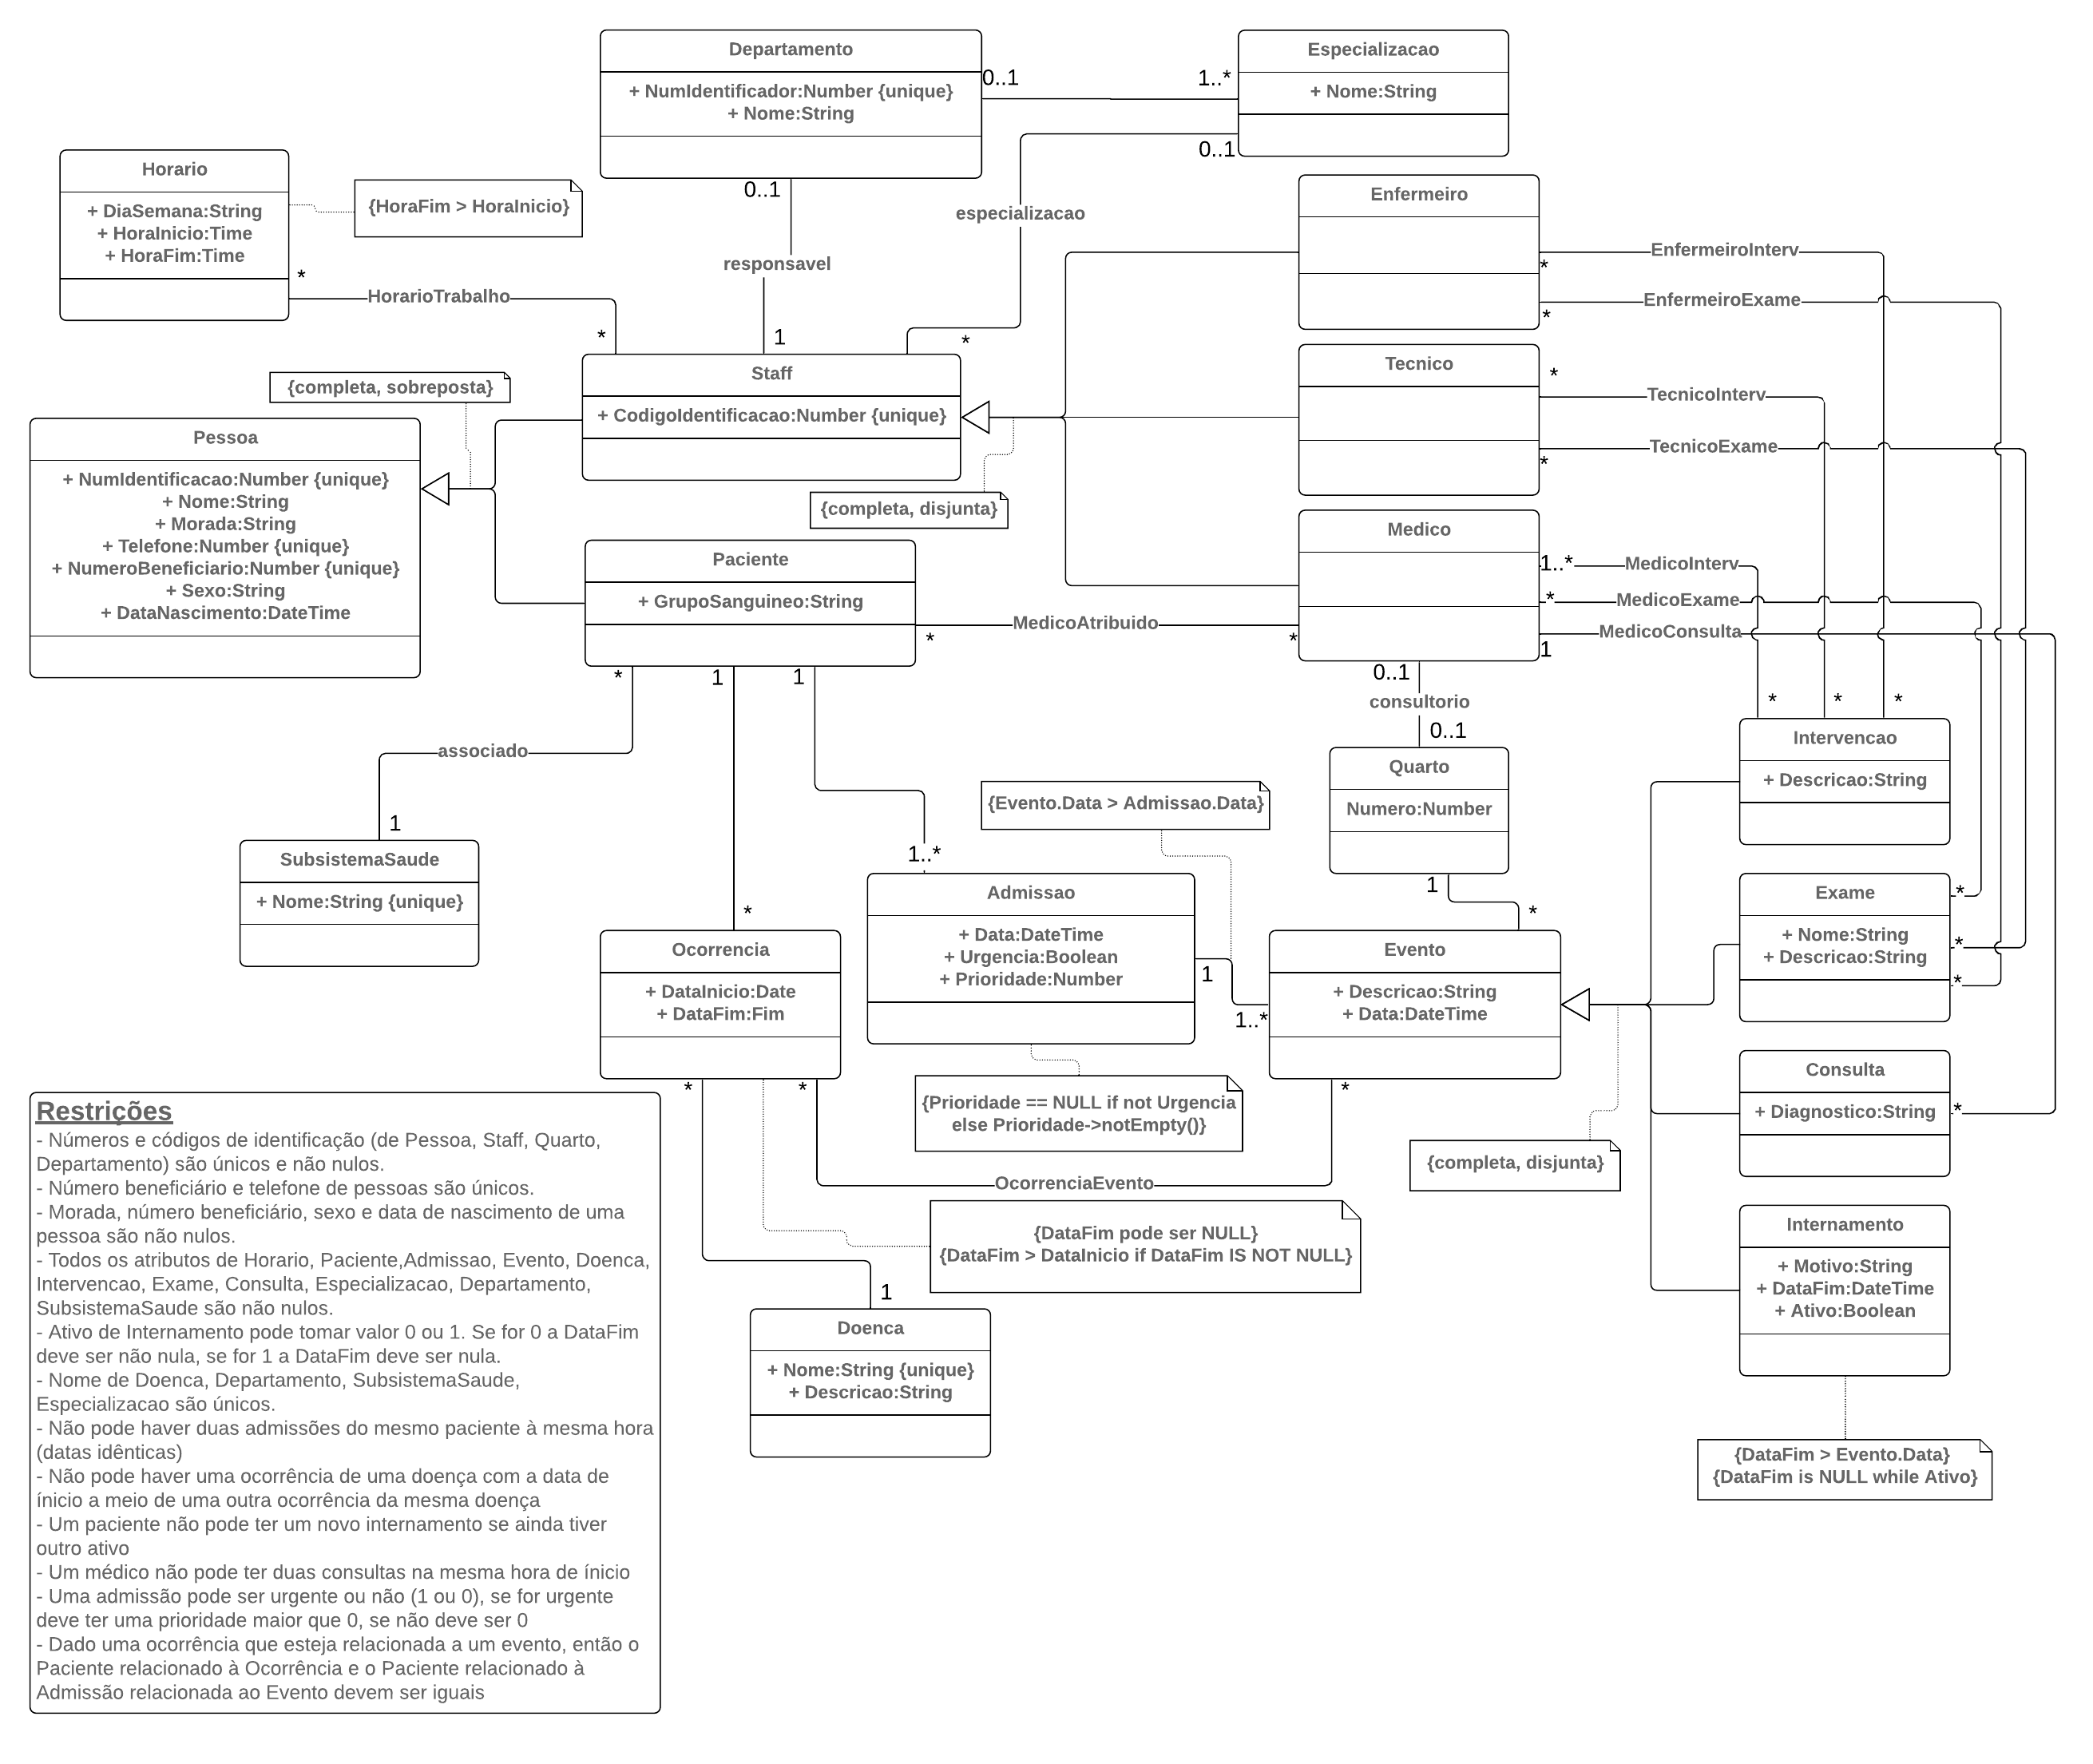
\includegraphics[width=1.1\linewidth, height=1.0\linewidth]{BDAD-UML.png}

\newpage
%----------------------------------------------------------------------------------------
%	CHAPTER 3 - Relational Model
%----------------------------------------------------------------------------------------
\chapter[Modelo Relacional][Modelo Relacional]{Modelo Relacional} \label{\thechapter}

\section{Classes}
\subsection{Classe Pessoa}
\begin{itemize}
	\item Pessoa(\underline{NumIdentificacao}, Nome, Morada, Localidade, CodigoPostal, Cidade, Pais, Telefone, NumeroBeneficiario, Sexo, DataNascimento)
\end{itemize}
\subsubsection{Classe Staff}
\begin{itemize}
	\item Staff(\underline{PessoaID}$\rightarrow$Pessoa, \underline{CodigoIdentificacao}, Especializacao$\rightarrow$Especializacao)
	\begin{itemize}
		\item Enfermeiro(\underline{StaffID}$\rightarrow$Staff)
		\item Tecnico(\underline{StaffID}$\rightarrow$Staff)
		\item Medico(\underline{StaffID}$\rightarrow$Staff, Consultorio$\rightarrow$Quarto)
	\end{itemize}
	\item Especializacao(\underline{Nome}, Departamento$\rightarrow$Departamento)
	\item Horario(\underline{HorarioID}, DiaSemana, HoraInicio, HoraFim)
	\item Departamento(\underline{NumIdentificador}, Nome, Responsavel$\rightarrow$Staff)
\end{itemize}
\subsubsection{Classe Paciente}
\begin{itemize}
	\item Paciente(\underline{PessoaID}$\rightarrow$Pessoa, GrupoSanguineo, SubsistemaSaude$\rightarrow$SubsistemaSaude)
	\item SubsistemaSaude(\underline{Nome})
\end{itemize}
\subsection{Classe Evento}
\begin{itemize}
	\item Admissao(\underline{AdmissaoID}, Data, Urgencia, Prioridade, Paciente$\rightarrow$Paciente)
	\item Doenca(\underline{Nome}, Descricao, Sintomas)
	\item Ocorrrencia(\underline{OcorrenciaID}, DataInicio, DataFim, Paciente$\rightarrow$Paciente, Doenca$\rightarrow$Doenca)
	\item Quarto(\underline{Numero})
	\item Evento(\underline{EventoID}, Descricao, Data, Admissao$\rightarrow$Admissao, Quarto$\rightarrow$Quarto)
	\begin{itemize}
		\item Intervencao(\underline{EventoID}$\rightarrow$Evento, Descricao)
		\item Exame(\underline{EventoID}$\rightarrow$Evento, Nome, Descricao)
		\item Consulta(\underline{EventoID}$\rightarrow$Evento, Diagnostico, Medico$\rightarrow$Medico)
		\item Internamento(\underline{EventoID}$\rightarrow$Evento, Motivo, DataFim, Ativo)
	\end{itemize}
\end{itemize}

\section{Associações}
\subsection{Associações muitos-para-muitos}
Associações relativas à classe Staff:
\begin{itemize}
	\item HorarioTrabalho(\underline{StaffID}$\rightarrow$Staff, \underline{HorarioID}$\rightarrow$Horario)
\end{itemize}

Associações relativas à classe Paciente:
\begin{itemize}
	\item MedicoAtribuido(\underline{PacienteID}$\rightarrow$Paciente, \underline{MedicoID}$\rightarrow$Medico)
\end{itemize}

Associações relativas à classe Evento:
\begin{itemize}
	\item EnfermeiroInterv(\underline{EnfermeiroID}$\rightarrow$Enfermeiro, \underline{IntervID}$\rightarrow$Intervencao)
	\item EnfermeiroExame(\underline{EnfermeiroID}$\rightarrow$Enfermeiro, \underline{ExameID}$\rightarrow$Exame)
	\item TecnicoInterv(\underline{TecnicoID}$\rightarrow$Tecnico, \underline{IntervID}$\rightarrow$Intervencao)
	\item TecnicoExame(\underline{TecnicoID}$\rightarrow$Tecnico, \underline{ExameID}$\rightarrow$Exame)
	\item MedicoInterv(\underline{MedicoID}$\rightarrow$Medico, \underline{IntervID}$\rightarrow$Intervencao)
	\item MedicoExame(\underline{MedicoID}$\rightarrow$Medico, \underline{ExameID}$\rightarrow$Exame)
	\item OcorrenciaEvento(\underline{OcorrenciaID}$\rightarrow$Ocorrencia, \underline{EventoID}$\rightarrow$Evento)
\end{itemize}

\subsection{Associações muitos-para-um}
Para este tipo de associações foi adotado o método de adicionar uma chave estrangeira para a relação "um" na relação "muitos".

\subsection{Associações um-para-um}
Para este tipo de associações foi adicionado uma chave estrangeira à relação que possuirá o menor número de tuplos, exceto nos casos em que essa relação poder ter esse elemento como nulo, nos casos em que ambos podem ser nulos, 

\section{Generalizações}
Quanto as generalizações, optou-se por usar o método E/R, criando uma relação para cada classe, e adicionando a chave da super-classe às subclasses.

\newpage
%----------------------------------------------------------------------------------------
%	CHAPTER 4 - Analysis of Functional Dependencies and Normal Forms
%----------------------------------------------------------------------------------------
\chapter[Análise de FDs e FNs][Análise de FDs e FNs]{Análise de Dependências Funcionais e Formas Normais} \label{\thechapter}

\section{Classes}
\subsection{Pessoa}


\section{Associações}

\newpage
%----------------------------------------------------------------------------------------
%	CHAPTER 5 - Restrictions
%----------------------------------------------------------------------------------------
\chapter[Restrições][Restrições]{Restrições} \label{\thechapter}

\section*{Pessoa}
\begin{itemize}
	\item cada pessoa tem um número de identificação único (\textbf{PRIMARY KEY})
	\item cada pessoa deve ter um nome, morada, localidade, código postal, cidade, país, número beneficiário, sexo e data nascimento (\textbf{NOT NULL})
	\item o números de telefone devem ser únicos (\textbf{UNIQUE})
\end{itemize}

\section*{Staff}
\begin{itemize}
	\item cada membro da staff tem um código identificação único, além do número de identificação único (\textbf{PRIMARY KEY})
	\item além disso, número de identificação (\textbf{PessoaID}) é chave estrangeira para Pessoa (\textbf{REFERENCES})
	\item não é possível eliminar uma pessoa enquanto houver staff mapeada para essa pessoa, mas pode-se alterar a pessoa que alterará na staff que a mapeia (\textbf{ON DELETE RESTRICT} e \textbf{ON UPDATE CASCADE})
	\item Especializacao é chave estrangeira para Especializacao, e tal será posta a \textbf{NULL} caso a Especializacao seja eliminada, em caso de alterações, as alterações seram feitas em toda a staff que mapeia essa especialização (\textbf{ON DELETE SET NULL} e \textbf{ON UPDATE CASCADE})
\end{itemize}

\subsubsection*{Enfermeiro}
\begin{itemize}
	\item cada enfermeiro tem o seu código de identificação (\textbf{StaffID}) que é chave estrangeira para Staff
	\item não é possível eliminar um membro da staff enquanto houver um enfermeiro mapeado para esse membro da staff, mas pode-se alterar a staff que alterará também no enfermeiro que a mapeia (\textbf{ON DELETE RESTRICT} e \textbf{ON UPDATE CASCADE})
	\item além disso, este código de identificação deve ser único (\textbf{PRIMARY KEY})
\end{itemize}

\newpage

\subsubsection*{Tecnico}
\begin{itemize}
	\item cada técnico tem o seu código de identificação (\textbf{StaffID}) que é chave estrangeira para Staff
	\item não é possível eliminar um membro da staff enquanto houver um técnico mapeado para esse membro da staff, mas pode-se alterar a staff que alterará também no técnico que a mapeia (\textbf{ON DELETE RESTRICT} e \textbf{ON UPDATE CASCADE})
	\item além disso, este código de identificação deve ser único (\textbf{PRIMARY KEY})
\end{itemize}

\subsubsection*{Medico}
\begin{itemize}
	\item cada médico tem o seu código de identificação (\textbf{StaffID}) que é chave estrangeira para Staff
	\item não é possível eliminar um membro da staff enquanto houver um médico mapeado para esse membro da staff, mas pode-se alterar a staff que alterará também no médico que a mapeia (\textbf{ON DELETE RESTRICT} e \textbf{ON UPDATE CASCADE})
	\item além disso, este código de identificação deve ser único (\textbf{PRIMARY KEY})
\end{itemize}

\section*{Especializacao}
\begin{itemize}
	\item cada especialização deve ter um nome único (\textbf{PRIMARY KEY})
	\item Departamento é chave estrangeira para Departamento
\end{itemize}

\section*{Horario}
\begin{itemize}
	\item cada horário tem um ID único (\textbf{PRIMARY KEY})
\end{itemize}

\end{document}
